\documentclass[conference]{assets/latex/IEEEtran}
\IEEEoverridecommandlockouts
% The preceding line is only needed to identify funding in the first footnote. If that is unneeded, please comment it out.
%Template version as of 6/27/2024

\usepackage{amsmath,amssymb,amsfonts}
\usepackage{algorithmic}
\usepackage{graphicx}
\usepackage{textcomp}
\usepackage{xcolor}
\usepackage[backend=biber,style=numeric]{biblatex}
\addbibresource{assets/latex/report.bib}

 \graphicspath{{assets/latex/}}

\begin{document}

\title{CS6524 Computer Vision Lab. 3\\ Structure from Motion}

\author{\IEEEauthorblockN{Edmund Phelan}
\IEEEauthorblockA{\textit{University of Limerick}\\
Student ID 23397179}
\and
\IEEEauthorblockN{Andrew Jaffray}
\IEEEauthorblockA{\textit{University of Limerick}\\
Student ID 23382163}
}

\maketitle

\begin{abstract}
We reconstruct a Bulbasaur figure from two phone videos: one with the camera
circling the figure (a) and one with the figure spinning in front of a still
camera (b). SIFT tracks give a pose for each frame pair, and PnP with bundle
adjustment joins all frames into one sparse model. Video a registers all 58
frames, with 0.27\,px median error and a closed 360$^\circ$ loop. Video b only
works at the true focal length, since one slow frame pair breaks the chain.
\end{abstract}

\section{Setup}
\begin{itemize}
\item \textbf{Object:} a Bulbasaur (Pokemon) figure standing on a printed
checkerboard on a table.
\item \textbf{Videos:} in video a the camera walks a full circle around the
figure. In video b the camera stays still and the figure is turned by hand.
\item \textbf{Camera:} an iPhone 15, with $K$ and $D$ from our Lab~2
calibration ($f \approx 623$\,px). That calibration used landscape frames, so we
rotate $K$ and $D$ to portrait: $f_x$ and $f_y$ swap, and so do $c_x$ and $c_y$.
\item \textbf{Preprocessing:} each video is resized from $1080\times1920$ to
$360\times640$ and every second frame is kept (about 15\,fps). This keeps each
file under 5\,MB.
\item \textbf{Frame sampling:} video a uses every 5th frame (58 frames), since
consecutive frames are only about 1$^\circ$ apart. Video b uses all 125 frames.
\item \textbf{Undistortion:} $D$ has large $k_2$ and $k_3$ terms that mostly
cancel. The net correction is still 17--19\,px at the image corners and zero at
the centre.
\end{itemize}

\section{Methodology}

\subsection{Features and Tracks}

We detect SIFT~\cite{lowe2004sift} keypoints in each frame (median 369 in a,
533 in b). Consecutive frames are matched with Lowe's ratio test (0.75), and
matches are kept one-to-one. RANSAC on the essential matrix (1\,px) then leaves
about 107 inliers per frame pair. Chaining these matches gives tracks. In total,
411 tracks in a and 980 in b span five or more frames. In video b we drop
matches that move less than 1\,px. Otherwise the static background outvotes the
spinning Pokemon figure.

\subsection{Pairwise Pose and Triangulation}\label{sec:pose}
Each essential matrix is decomposed into a rotation $R$ and translation $t$.
The cheirality check picks the one solution that puts the points in front of
both cameras~\cite{foundationsCVbook}. The scale of $t$ is unknown, so we set
$|t|=1$. In video a the first and last pairs fail this check, because the
camera barely moves before and after the walk around the Pokemon. We then place frame $i$ at $K[I|0]$ and frame $i{+}1$
at $K[R|t]$ and triangulate the inliers. Points behind either camera are
dropped. Reprojecting the points into both frames gives a median error of
0.12--0.16\,px in every run of Table~\ref{tab:sens}. This includes runs that
later collapse. With only two views and a 1\,px RANSAC threshold, the error is
small by construction. It therefore says little about the final reconstruction.

\subsection{N-Frame Reconstruction}\label{sec:nframe}
% EDDIE (~1 paragraph), reconstruct + bundle_adjust in sfm.py:
%  - Init pair: first pair with >= 50 shared tracks and >= 3 deg rotation (why not
%    frames 0-1: b barely moves at the start, 0.1 deg).
%  - Each later frame: PnP-RANSAC on tracks that already have a 3D point -> pose in the
%    same world frame and scale; then triangulate new tracks (>= 1 deg parallax, < 4 px).
%  - Local bundle adjustment of the last 8 poses every 5 frames, one global BA at the end,
%    Huber loss f_scale = 2 px (why 2 px and not 1 px: your synthetic test, 4 vs 0.3 deg)
%    \cite{foundationsCVbook}.
%  - Output: sparse cloud coloured from the frames -> the PLY files.

\section{Results}
For the sensitivity analysis we scale $f_x$ and $f_y$ by 0.8, 1.0 and 1.2. The
scaled $K$ is used in every step, including undistortion. Each factor is run
with and without undistortion, giving six runs per video. Table~\ref{tab:sens}
reports the frames registered in Section~\ref{sec:nframe}, the sparse points,
their median reprojection error and the summed rotation between consecutive
cameras. A full turn around the Bulbasaur should give about 360$^\circ$. The
reference run a\_10u registers all 58 frames with 0.27\,px error and
369$^\circ$ of rotation. Two groups of runs collapse: a\_08d registers only 9
frames, and video b registers at most 66 of 125 frames at factors 0.8 and 1.2.

\begin{table}[t]
\caption{Sensitivity analysis: 12 runs (focal factor $\times$ undistortion)}
\begin{center}
\begin{tabular}{|l|c|c|c|c|}
\hline
\textbf{Run} & \textbf{Registered} & \textbf{Points} & \textbf{Err. (px)} & \textbf{Rot. ($^\circ$)} \\
\hline
a\_08u & 54/58 & 1902 & 0.52 & 392.5 \\
a\_10u & 58/58 & 2455 & 0.27 & 369.3 \\
a\_12u & 58/58 & 2861 & 0.37 & 399.7 \\
a\_08d & 9/58 & 143 & 0.18 & 38.1 \\
a\_10d & 58/58 & 2766 & 0.27 & 375.0 \\
a\_12d & 58/58 & 2711 & 0.41 & 402.8 \\
\hline
b\_08u & 36/125 & 1882 & 0.23 & 58.9 \\
b\_10u & 122/125 & 4704 & 0.39 & 362.4 \\
b\_12u & 41/125 & 2250 & 0.25 & 76.6 \\
b\_08d & 66/125 & 3213 & 0.32 & 136.7 \\
b\_10d & 124/125 & 6753 & 0.26 & 375.0 \\
b\_12d & 43/125 & 2471 & 0.23 & 78.6 \\
\hline
\end{tabular}
\label{tab:sens}
\end{center}
% ANDREW: re-check these against out/metrics.csv after the final run if any code changes.
\end{table}

% EDDIE: Figure 1, top-down view of the recovered camera centres + sparse cloud for
% a_10u (closed loop around the object) and b_10u (uneven arc). Save as
% assets/latex/trajectory.png, then uncomment the block below.
% \begin{figure}[t]
% \centerline{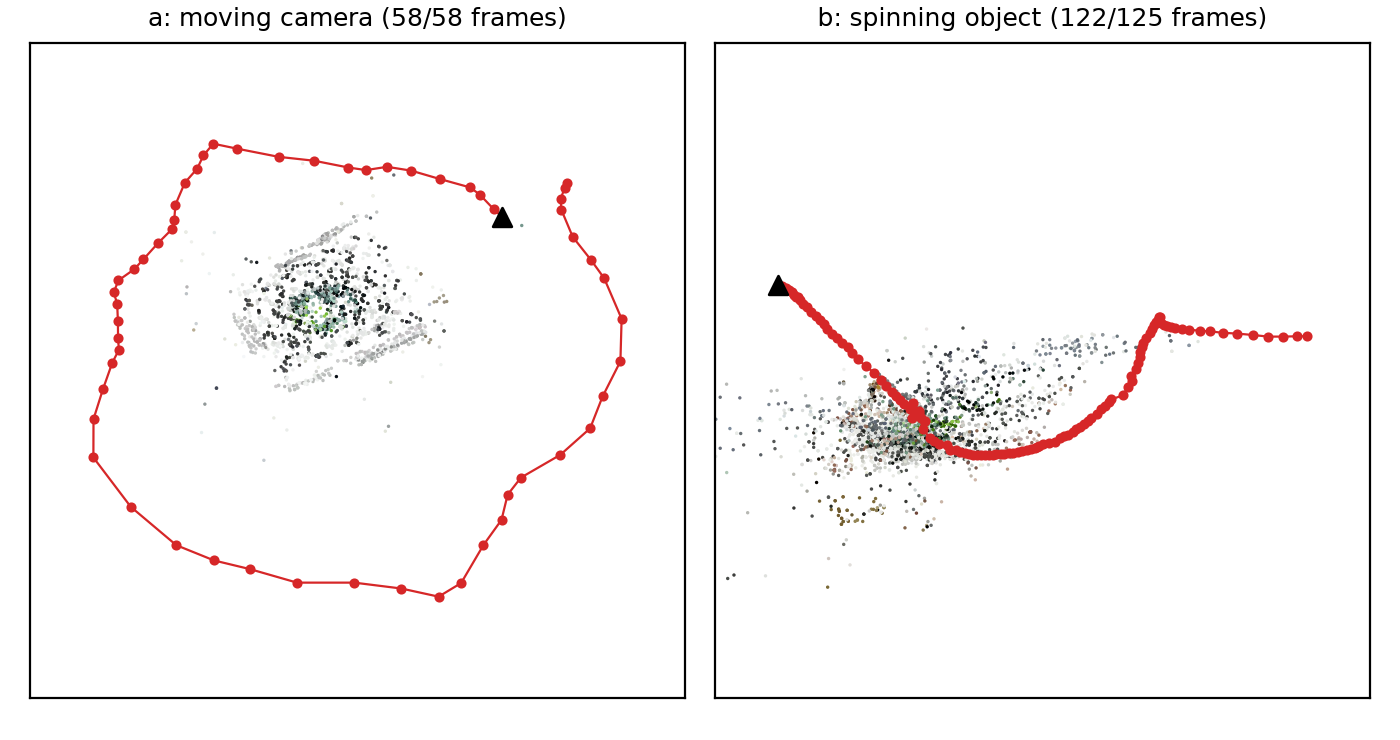
\includegraphics[width=\columnwidth]{trajectory.png}}
% \caption{Top view of camera centres (red) and sparse points for videos a (left) and b (right).}
% \label{fig:traj}
% \end{figure}

\section{Discussion and Failure Analysis}
% EDDIE, paragraph 1: sensitivity of video a (focal length + distortion).
%  - a tolerates a wrong focal length: all/most frames registered at 0.8 and 1.2, but the
%    summed rotation inflates (369 -> 392-403 deg): wrong f distorts angles, so the loop
%    no longer closes.
%  - Distortion matters in combination: a_10d is fine (375 deg), a_08d collapses (9/58).
%    Explain why error in f + uncorrected k1..k3 pushes PnP past its tolerance.

% EDDIE, paragraph 2: failure of video b.
%  - Only the true focal length survives: 36-43/125 frames at 0.8 and 1.2.
%  - Single point of failure at frame pair 36: object nearly pauses (hand repositioning?).
%    With the 1 px motion filter only 35 inliers remain there (vs ~150) and 4-9 tracks span
%    it, so PnP loses the chain. 0.5 px keeps 146 inliers / ~72 tracks.
%  - Camera path (Fig. 1) is an arc, not a circle, even in the best run: the
%    spinning-object = orbiting-camera equivalence only holds if nothing static is matched.
%  - Supporting evidence: b_10u registers 122/125 frames on macOS but 35/125 in the CI
%    Docker image (different OpenCV build) -> b sits on a knife edge.

We also tried a dense step but left it out of the final pipeline. It used
Farneback optical flow between posed frame pairs and triangulated every pixel
with the poses from Section~\ref{sec:nframe}. Depth from a single pair was very
noisy. We measured noise as the distance from each dense point to the nearest
sparse point. Keeping only voxels confirmed by three frame pairs cut the 90th
percentile of this distance from about 100 to about 5 sparse spacings. The
result for video a showed the checkerboard and the Bulbasaur. Video b was
unusable, because its camera poses were already wrong.

With more time, we would make the following changes:
\begin{itemize}
\item Match each frame to frame $i{+}2$ as well. One weak pair could then no
longer break the tracks in video b.
\item Match the last frames back to the first to close the loop. This would
pull the summed rotation from 369$^\circ$ back to 360$^\circ$.
\item Refine $f_x$ and $f_y$ inside bundle adjustment. This targets the focal
length errors directly.
\item Mask the Bulbasaur in video b instead of filtering by motion.
\end{itemize}

% Add \cite{...} in the text; unused entries are not printed.
% Available keys: foundationsCVbook, lowe2004sift
\printbibliography

\end{document}
